        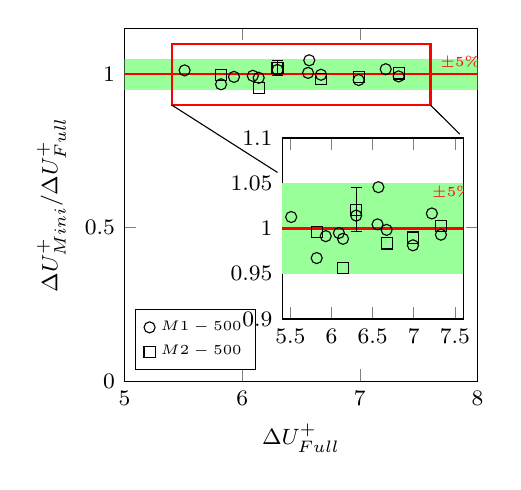
\begin{tikzpicture}[]
        \centering
        \begin{axis}[
            ylabel={$\Delta U_{\text{Mini}}^+/\Delta U_{\text{Full}}^+$},
            xlabel={$\Delta U_{\text{Full}}^+$},
            ymin=0, %ymax=1.2,
			xmax=8,
			xmin=5,
			%xtick={-2,-1.5,...,-0.4},
            width=.5\linewidth,
            height=.5\linewidth,
            label style={font=\footnotesize},
            legend style={font=\tiny,anchor=south west},
                        legend pos=south west,
            tick label style={font=\footnotesize}
            ]
			\addplot [
            black,only marks,mark=o,
            ]
            coordinates{
            (6.67,6.66/6.67)
            (6.56,6.59/6.56)
            (6.30,6.39/6.30)
            (5.93,5.88/5.93)
            (7.33,7.28/7.33)
            (7.22,7.34/7.22)
            (6.99,6.86/6.99)
            (6.57,6.87/6.57)
            (6.14,6.07/6.14)
            (6.09,6.06/6.09)
            (5.82,5.63/5.82)
            (5.51,5.58/5.51)
            };
			\addlegendentry{$M1-500$}
			\addplot [
            black,only marks,mark=square,
            ]
            coordinates{
            (6.67, 6.56/6.67)
            (6.30, 6.43/6.30)
            (7.33,7.35/7.33)
            (6.99,6.92/6.99)
            (6.14,5.87/6.14)
            (5.82,5.80/5.82)
            };
			\addlegendentry{$M2-500$}%
			

%						\addplot [
%            gray,only marks,mark=square,
%            ]
%            coordinates{
%            (6.30, 6.46/6.30)
%            (6.30, 6.42/6.30)
%            (6.30, 6.56/6.30)
%            (6.30, 6.58/6.30)
%            (6.30, 6.58/6.30)
%            (6.30, 6.19/6.30)
%            (6.30, 6.54/6.30)
%            (6.30, 6.30/6.30)
%            };
%			\addlegendentry{$G24M2-500s$}
			 \fill[color=green!40,opacity=40] (0,1.05) -- (9,1.05) -- (9,0.95) -- (0,0.95) -- cycle;
			 			%\fill[color=yellow!40,opacity=40] (0,0.18) -- (9,9.18) -- (9,8.82) -- (0,-0.18) -- cycle;
			 		
						\addplot [
            red,thick,solid,mark=square,
            ]
            coordinates{
            (0, 1)
            (9, 1)
            };
            \draw[color=red,thick] (5.4, 0.9) rectangle (7.6, 1.1);
			\node[red,right] at (axis cs: 7.6,1.04) {\tiny $\pm5\%$};
						\addplot[
        only marks,
        mark=square,
        black,
        error bars/.cd, y dir=both, y explicit,
    ] plot coordinates {
                    (6.30, 6.43/6.30)+=(0, 0.1539/6.30) -=(0, 0.1539/6.30)
    };
        \coordinate (AR1) at (5.4, 0.9);
        \coordinate (AR2) at (6.3, 0.68);
        \coordinate (AR3) at (7.6, 0.9);
        \coordinate (AR4) at (7.85, 0.805);
         \draw[-] (AR1) -- (AR2);
         \draw[-] (AR3) -- (AR4);
        \end{axis}
        
                \begin{axis}[
            %ylabel={$\frac{\Delta U_{Mini}^+}{\Delta U_{Full}^+}$},
            %xlabel={$\Delta U_{Full}^+$},
            ymin=0.9,ymax=1.1,
			xmax=7.6,
			xmin=5.4,
			%xtick={-2,-1.5,...,-0.4},
            width=.32\linewidth,
            height=.32\linewidth,
            label style={font=\footnotesize},
            tick label style={font=\footnotesize},
            at={(0.165\linewidth,0.065\linewidth)}
            ]
			\addplot [
            black,only marks,mark=o,
            ]
            coordinates{
            (6.67,6.66/6.67)
            (6.56,6.59/6.56)
            (6.30,6.39/6.30)
            (5.93,5.88/5.93)
            (7.33,7.28/7.33)
            (7.22,7.34/7.22)
            (6.99,6.86/6.99)
            (6.57,6.87/6.57)
            (6.14,6.07/6.14)
            (6.09,6.06/6.09)
            (5.82,5.63/5.82)
            (5.51,5.58/5.51)
            };
			\addplot [
            black,only marks,mark=square,
            ]
            coordinates{
            (6.67, 6.56/6.67)
            (6.30, 6.43/6.30)
            (7.33,7.35/7.33)
            (6.99,6.92/6.99)
            (6.14,5.87/6.14)
            (5.82,5.80/5.82)
            };
%						\addplot [
%            gray,only marks,mark=square,
%            ]
%            coordinates{
%%            (6.30, 6.46/6.30)
 %           (6.30, 6.42/6.30)
 %           (6.30, 6.56/6.30)
 %           (6.30, 6.58/6.30)
 %           (6.30, 6.58/6.30)
 %           (6.30, 6.19/6.30)
 %           (6.30, 6.54/6.30)
 %           (6.30, 6.30/6.30)
 %           };

			 \fill[color=green!40,opacity=40] (0,1.05) -- (9,1.05) -- (9,0.95) -- (0,0.95) -- cycle;
			 			%\fill[color=yellow!40,opacity=40] (0,0.18) -- (9,9.18) -- (9,8.82) -- (0,-0.18) -- cycle;
						\addplot [
            red,thick,solid,mark=square,
            ]
            coordinates{
            (0, 1)
            (9, 1)
            };
			\node[red,right] at (axis cs: 7.1,1.04) {\tiny $\pm5\%$};
						 						\addplot[
        only marks,
        mark=square,
        black,
        error bars/.cd, y dir=both, y explicit,
    ] plot coordinates {
                    (6.30, 6.43/6.30)+=(0, 0.1539/6.30) -=(0, 0.1539/6.30)
    };
        \end{axis}
        \end{tikzpicture}